\documentclass[screen, aspectratio=43]{beamer}
\usepackage[T1]{fontenc}
\usepackage[utf8]{inputenc}

% Use the NTNU-temaet for beamer 
% \usetheme[style=ntnu|simple|vertical|horizontal, 
%     language=bm|nn|en, 
%     smalltitle, 
%     city=all|trondheim|alesund|gjovik]{ntnu2017}
\usetheme[style=ntnu,language=en]{ntnu2017}

\usepackage[english]{babel}
\usepackage[style=numeric,backend=biber,natbib=false,sorting=none]{biblatex}

\title[AP-intro]{MCT4048: Audio Programming}
\subtitle{Introduction}
\author[A. Xamb{\'o}]{Anna Xamb{\'o}}
\institute[NTNU]{Department of Music, NTNU}
\date{15 January 2015}
%\date{} % To have an empty date

\addbibresource{../ap.bib} % Add bibliography database

% Set the reference style to numeric.
% See here: http://tex.stackexchange.com/questions/68080/beamer-bibliography-icon
\setbeamertemplate{bibliography item}[text] 

% Set bibliography fonts to a small size.
\renewcommand*{\bibfont}{\footnotesize}

\begin{document}

\begin{frame}
  \titlepage
\end{frame}

% Alternatively, special title page command to get a different background
% \ntnutitlepage

%\begin{frame}
%\frametitle{Announcements}
%\begin{itemize}
%{\scriptsize 
%\item Team working: discussion how to do it this semester.
%\item Micro:bits arrived!
%\item New teacher member in Trondheim: Welcome Daniel Formo!
%\item Reminder -- Registration deadline (class+exam) and payment semester fee: February 1!
%\item Elective courses: Need to inform Stein, Terje or Maj first. Study plan: 30 CTS in 2 years.
%\item Program board: we need a student representative in Oslo.
%\item Safe space for all: code of conduct.
%\item January 30: Girls geek dinner, 18:45-19:15 network music concert?
%\item Trondheim: 2 prospective students: CoP, volunteers as student contact points?
%\item Pamela Z in Oslo 4.4.19: knowledge transfer Trondheim video streaming team (blog post?) 
%\item WoNoMute: calendar in Canvas.
%\item New MCT website: how to update content.
%}
%\end{itemize}
%\end{frame}
%

\begin{frame}
\frametitle{Warm-up activity: paper discussion}
\textbf{Task}: In the context of the topics discussed in the article, be ready to discuss in class your favourite computer music programming language (it could be one of the languages listed in the article, or another one). 
\begin{itemize}
\item What are the advantages and limitations?
\item How do they process events, gestures and sounds?
\item To what extent it is a general-purpose vs. task specific programming language?
\end{itemize}
\hfill \break
\textbf{Reference}: Dannenberg (2018). Languages for Computer Music. Frontiers in Digital Humanities, 5, 26.\\
%\url{https://www.frontiersin.org/articles/10.3389/fdigh.2018.00026/full\#h2}
\end{frame}
%
\begin{frame}
\frametitle{Syllabus}
\url{https://uio.instructure.com/courses/17406/pages/syllabus}
\end{frame}
%
\begin{frame}
\frametitle{Why Web Audio API?}
\begin{itemize}
\item It is written in one of the modern programming languages.
\item It is easy to sketch ideas and get prototypes built.
\item It is easy to test, implement, and distribute.
\item It showcases the fundamental concepts of audio programming.
\item It gives room for artistic expression.
\item It is an employable skill.
\item We will be hosting the Web Audio Conference 2019 at NTNU in Trondheim!
\end{itemize}
\end{frame}
%
\begin{frame}
\frametitle{Web Audio API?}
\begin{figure}
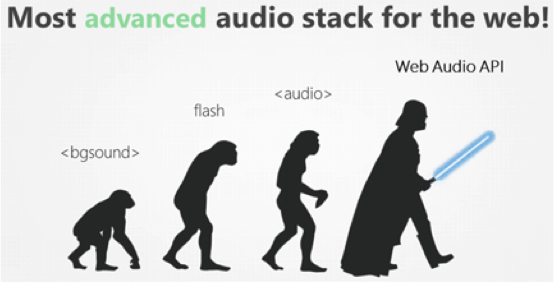
\includegraphics[scale=0.3]{img/advanced-web-audio.jpg}
{\\ \tiny Image source: http://www.sitepoint.com}\\
\end{figure}
High-level JavaScript API for processing and synthesizing audio in web applications.
\begin{itemize}
\item Cross-browser way of playing audio on the Web.
\item Native support for audio playback in all modern browsers.
\item Support of tasks found in modern desktop audio production applications.
\end{itemize}
\end{frame}
%
\begin{frame}
\frametitle{Pseudocode}
\begin{itemize}
\item It is an informal high-level description of the operating principle of a computer program or other algorithm. (Wikipedia)
\item It omits machine-level information (e.g. variable declarations).
\item It should be easy to understand.
\item It is an efficient and environment-independent description of the key principles of an algorithm.
\end{itemize}
\end{frame}
%
\begin{frame}
\frametitle{Exercise: Pseudocode}

\textbf{Task}: Write the program in pseudocode of a sampler that plays 4 sound samples when pressing 'a', 'x', 'd' and 'w' respectively. Add a key that switches between looping and not looping the current sound. Optionally, add 4 different effects when pressing four other keys. Consider loading the sounds first. Report back to the class the result and the challenges faced when writing the algorithm in pseudocode. \\
\hfill \break
\textbf{Reference}: \url{https://en.wikipedia.org/wiki/Pseudocode}\\
%\url{https://www.frontiersin.org/articles/10.3389/fdigh.2018.00026/full\#h2}
\end{frame}
%
%\begin{frame}
%\frametitle{}
%Time for GitHub and the MCT blog...
%\end{frame}
%
%\begin{frame}
%  \frametitle{References}
%  \printbibliography
%\end{frame}
%
\end{document}
